\appendix

\section{Exposed malicious exit relays}
\label{sec:malicious-relays}
Table~\ref{tab:exitmap-dataset} provides an overview of our second dataset, 251
bad exit relays that we discovered between August 2014 and January 2016.  We
believe that all single relays in the dataset were isolated incidents while sets
of relays constituted Sybil groups.  Sybil groups marked with the symbols
$\dagger$, $\ddagger$, and $\mathsection$ were run by the same attacker.

\rowcolors{1}{}{gray!10}

\begin{table*}
\small
\centering
\begin{tabularx}{\textwidth}{r c X}
\hline
\textbf{Discovery} & \textbf{\# of relays} & \textbf{Attack description} \\
\hline
% Message-ID: <20140811014615.GB23748@nymity.ch>
Aug 2014 & 1 & The relay injected JavaScript into returned HTML.  The script
embedded another script from the domain fluxx.crazytall.com---not clearly
malicious, but suspicious. \\

% Message-ID: <20140831153809.GA1799@nymity.ch>
Aug 2014 & 1 & The relay injected JavaScript into returned HTML.  The script
embedded two other scripts, jquery.js from the official jQuery domain, and
clr.js from adobe.flashdst.com.  Again, this was not necessarily malicious, but
suspicious. \\

% Message-ID: <20140920132357.GC8751@nymity.ch>
Sep 2014 & 1 & The exit relay routed traffic back into the Tor network, i.e., we
observed traffic that was supposed to exit from relay $A$, but came from relay
$B$.  The system presented by Ling et al. behaves the same~\cite{Ling2015a};
the authors proposed to run intrusion detection systems on Tor traffic by
setting up an exit relay that runs an NIDS system, and routes the traffic back
into the Tor network after having inspected the traffic. \\

% Message-ID: <20141021133016.GA11247@nymity.ch>
Oct 2014 & 1 & The relay injected JavaScript into returned HTML. \\

% Message-ID: <20141021133016.GA11247@nymity.ch>
Oct 2014 & 1 & The relay ran the MitM tool sslstrip~\cite{sslstrip}, rewriting
HTTPS links to unencrypted HTTP links in returned HTML. \\

% Message-ID: <20141025182433.GA23244@nymity.ch>
Oct 2014 & 1 & Same as above. \\

% Message-ID: <20150109195428.GA29115@nymity.ch>
Jan 2015 & 23$\ddagger$ & Blockchain.info's web server redirects its
users from HTTP to HTTPS.  These relays tampered with blockchain.info's redirect
and returned unprotected HTTP instead---presumably to sniff login credentials. \\

Jan 2015 & 1 & The relay used OpenDNS as DNS resolver and had the web site
category ``proxy/anonymizer'' blocked, resulting in several inaccessible web
sites, including torproject.org. \\

% Message-ID: <20150210154109.GD10777@nymity.ch>
Feb 2015 & 1 & The relay injected a script that attempted to load a resource
from the now inaccessible torclick.net.  Curiously, torclick.net's front page
said ``We place your advertising materials on all websites online.  Your ads
will be seen only for anonymous network TOR [sic] users.  Now it is about 3
million users. The number of users is always growing.'' \\

Feb 2015 & 17$\ddagger$ & Again, these relays tampered with HTTP redirects of
Bitcoin web sites.  Interestingly, the attack became more sophisticated; these
relays would only target connections whose HTTP headers resembled Tor Browser.
\\

% Message-ID: <20150311131506.GE23215@nymity.ch>
Mar 2015 & 18$\ddagger$ & Same as above. \\

% Message-ID: <20150311125831.GD23215@nymity.ch>
Mar 2015 & 1 & The relay injected JavaScript and an iframe into the returned
HTML.  The injected content was not clearly malicious, but suspicious. \\

% Message-ID: <20150423004031.GA11395@nymity.ch>
Apr 2015 & 70$\dagger$ & These exit relays transparently rewrote onion domains
in returned HTML to an impersonation domain.  The impersonation domain looked
identical to the original, but had different Bitcoin addresses.  We believe that
this was attempt to trick Tor users into sending Bitcoin transactions to
phishing addresses. \\

% Message-ID: <20150630022923.GA2340@nymity.ch>
Jun 2015 & 55$\dagger$ & Same as above. \\

% Message-ID: <20150804202838.GA4774@nymity.ch>
Aug 2015 & 4$\dagger$ & Same as above. \\

% Message-ID: <20150908174557.GG8901@nymity.ch>
Sep 2015 & 1 & The relay injected an iframe into returned HTML that would load
content that made the user's browser participate in some kind of mining
activity. \\

% Message-ID: <20151116164403.GL10892@nymity.ch>
Nov 2015 & 1 & The relay ran the MitM tool sslstrip. \\

% Message-ID: <20151117150055.GA25187@nymity.ch>
Nov 2015 & 8$\dagger$ & Same as the relays marked with a $\dagger$. \\

% Message-ID: <20151213025807.GB20685@nymity.ch>
Dec 2015 & 1$\mathsection$ & The relay ran the MitM tool sslstrip. \\

% Message-ID: <20151214230014.GA27729@nymity.ch>
Dec 2015 & 1$\mathsection$ & Same as above. \\

% Message-ID: <20160112033141.GA499@nymity.ch>
Jan 2016 & 43$\dagger$ & Same as the relays marked with a $\dagger$. \\
\hline
\end{tabularx}
\caption{An overview of our second dataset, 251 malicious exit relays that we
discovered using exitmap.  We believe that Sybil groups marked with an
$\dagger$, $\mathsection$, and $\ddagger$ were run by the same adversary.}
\label{tab:exitmap-dataset}
\end{table*}

\section{Supporting diagrams}
Figure~\ref{fig:default-sybils-uptime} shows the uptime matrix for the
``default'' Sybil group for October 2015.  Matrix rows represent consensuses and
columns represent relays.  As a result, a single pixel shows if a given relays
was online (black pixel) or offline (white pixel) in a given consensus.  The
matrix shows that many relays exhibit a diurnal uptime pattern.

\begin{figure}[h]
	\centering
	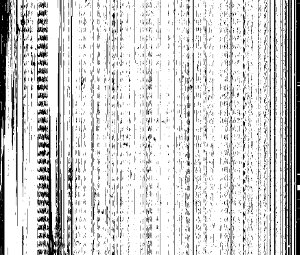
\includegraphics[width=0.8\linewidth]{diagrams/default-sybils-2015-10.jpg}
	\caption{Uptimes for the ``default'' Sybil group for October 2015.  Many
	relays exhibit a diurnal pattern, suggesting that the relays were powered
	off regularly.}
	\label{fig:default-sybils-uptime}
\end{figure}
